\documentclass[twocolumn,notitlepage,prl,superscriptaddress,showpacs]{revtex4-1}
\usepackage{hyperref}
\usepackage[usenames,dvipsnames]{color}
\usepackage{amsmath}
\usepackage[english]{babel}
\usepackage{amssymb}
\usepackage{graphicx}
\usepackage{epstopdf}
%\usepackage{lineno}
\usepackage{tabularx}
\usepackage{multirow}
\usepackage[]{todonotes}
\newcommand{\fedortodo}[2]{\todo[inline,backgroundcolor=orange!20!white]{\color{BlueViolet}{{\bf \it by: #1}:  {\bf Fedor:} #2}}}
\newcommand{\jamestodo}[2]{\todo[inline,backgroundcolor=orange!20!white]{\color{Maroon}{{\bf \it by: #1}: {\bf James:} #2}}}

%\setlength\linenumbersep{2pt}
\newcommand*\Eval[3]{\left.#1\right\rvert_{#2}^{#3}}
\begin{document}
%\linenumbers
\title{Controlled study of the Fermi/non-Fermi liquid crossover in the half-filled 2D Hubbard Model}

\author{Fedor \v{S}imkovic IV.}
\affiliation{Department of Physics, King’s College London, Strand, London WC2R 2LS, UK}
\author{Evgeny Kozik}
\affiliation{Department of Physics, King’s College London, Strand, London WC2R 2LS, UK}
\author{Youjin Deng}
\affiliation{Hefei National Laboratory for Physical Sciences at Microscale and Department of Modern Physics, University of Science and Technology of China, Hefei, Anhui 230026, China}
\author{N. V. Prokof'ev}
\affiliation{Department of Physics, University of Massachusetts, Amherst, MA 01003, USA}
% * <jpfleblanc@gmail.com> 2016-06-13T15:10:41.276Z:
%
% ^.
\affiliation{Russian Research Center ``Kurchatov Institute'', 123182 Moscow, Russia}
\author{B.V. Svistunov}
\affiliation{Department of Physics, University of Massachusetts, Amherst, MA 01003, USA}
\affiliation{Russian Research Center ``Kurchatov Institute'', 123182 Moscow, Russia}
\author{Emanuel Gull}
\affiliation{Department of Physics, University of Michigan, Ann Arbor, Michigan 48109, USA} 
\author{J. P. F. LeBlanc}
\affiliation{Department of Physics and Physical Oceanography, Memorial University of Newfoundland, St. John's, Newfoundland \& Labrador A1B 3X7, Canada} 

\collaboration{The Simons Collaboration on the Many-Electron Problem}

\date{\today}

\begin{abstract}
We study the Fermi/non-Fermi liquid crossover of the 2D Hubbard model at half filling and low temperatures in the thermodynamic limit using Self-energy Determinantal Diagrammatic Monte-Carlo ($\Sigma$DDMC) and Dynamical Cluster Approximation (DCA). We compute the imaginary part of the self energy, which we use as a metric for the Fermi/non-Fermi liquid crossover defined by $\rm{Im}\Sigma_k (i\omega_0) =\rm{Im}\Sigma_k (i\omega_1)$.
This is possible due to algorithmic advances in $\Sigma$DDMC that allow the computation of the Feynman diagrammatic series for the self-energy up to high diagram orders ($\sim$12) which permits the use of analytic continuation methods.  Our results suggest that the critical values of $U\to 0$ at $T\to 0$ and that the momentum differentiated anti-nodal and nodal points merge.  We verify results at high temperatures with large cluster DCA.  
\end{abstract}

\maketitle
%\listoftodos

\section{Introduction}

 The interaction driven metal-insulator transition has been for many years a problem of central focus for the field of strongly correlated electron systems.\cite{park:2008,georges:1996} Of particular impact has been the observation of such a transition within the single band Hubbard model in two-dimensions, the quintessential model of strongly correlated systems.\cite{schaefer:2015,  benchmark:2015}
For this model the role of non-perturbative numerical methods has been particularly important, such as the dynamical mean field theory and related cluster extensions.\cite{Maier05,georges:1996}  Those methods have observed metal to insulator transitions for strong interaction, and metallic phases for weakly interacting systems that persist to low temperatures. Key examples of such are studies performed at low temperatures ($\beta t=100$) on small (12 site) real-space clusters\cite{park:2008} that identified a critical value of interaction strength, $U_n/t$, above which the metallic system becomes insulating, and below which it has metallic characteristics with Fermi liquid renormalization parameters. It was also shown that short-range spin fluctuations are the reason for a decrease in critical interaction strength as well as a reverse of slope as compared to DMFT results.

\textbf{We need a paragraph right here that explains where the analytic formulation of $U_n\propto e^{b/\sqrt{U}}$ comes from. This should tie into the next paragraph.} 

 Recent advances and diagrammatic extensions of the dynamical mean field theory
provided a new tool-set for studying this problem and cast some doubt on previous numerical results.\cite{schaefer:2015,vanloon:2018} A study using the dynamical vertex approximation  (D$\Gamma$A) and lattice Quantum Monte Carlo (QMC) \cite{schaefer:2015} suggested that at low enough temperatures the Fermi surface always becomes gapped, even for weak interaction strength. It seems that the correlations that lead to insulating behavior at low temperatures are long range correlations that are explicitly truncated in cluster DMFT calculations on small systems. Therefore the physics observed in small system calculations may be both quantitatively and qualitatively distinct from the thermodynamic limit (TDL).\cite{benchmark:2015} However, quantitative results have yet to be rigorously obtained, for example the results obtained in Ref.~\cite{schaefer:2015} shows that the finite $T$ crossover exhibits a linear relation between $T$ and $U$ which is in contrast to an onset predicted from weak-coupling arguments $\propto e^{b/\sqrt{U}}$. [NEED REF]

 In this manuscript, we resolve these issues in the 2D Hubbard model at half-filling by utilizing the newly developed diagrammatic algorithm $\Sigma$DDMC \cite{simkovic2017determinant}. The method samples all possible diagram topologies by means of determinants \cite{burovski2006critical} and uses a recursive scheme \cite{rossi2017determinant} to filter out only one-particle irreducible self-energy diagrams. This permits the computation of a factorial number of Feynman diagram topologies in exponential time and improves the Monte Carlo variance due to symmetrization over topologies and internal vertex variables. From this we present the Fermi/non-Fermi liquid crossover diagram of the 2D Hubbard model in the thermodynamic limit. 
 We find two crossovers; a low temperature crossover to the state with a quasigap in the single-particle spectrum and a standard high-temperature crossover to the thermal liquid state. We demonstrate that the extremely slow convergence of observables as a function of finite size scaling is the source of past inconsistencies in numerical results\cite{vanloon:2018} and we further illustrate this issue through comparison of $\Sigma$DDMC in the TDL to $\Sigma$DDMC on finite lattices as well as results from the dynamical cluster approximation (DCA).

%%%%%%%%%%%%%%
\section{Model and Methods}

 We study the single-band Hubbard model in two-dimensions with nearest neighbor hopping,
\begin{equation}
H = \sum_{k,\sigma} \left(\epsilon_{k} -\mu\right)c_{k\sigma}^\dagger c_{k\sigma}+U\sum_i n_{i\uparrow}n_{i\downarrow},
\label{H}
\end{equation}
where $\mu$ is the chemical potential, $k$ momentum, $i$ labels of sites in real-space, $U$ the interaction, and the dispersion is given by
$\epsilon_k=-2t\left[\cos(k_x)+\cos(k_y)\right].$

 We seek solutions in the TDL and to make connection to dynamical mean-field theory (DMFT). To accomplish this, we employ two numerical techniques: Self-energy Determinant Diagrammatic Monte Carlo ($\Sigma$DDMC) and dynamical cluster approximation (DCA). 

In the language of Fermi liquid theory, an interacting system has a quasiparticle residue  defined at the Fermi level which contains a term proportional to $\lim\limits_{\omega\to 0}\frac{\partial \rm{Re}\Sigma_k (\omega)}{\partial \omega}$.  When on the 
Matsubara axis, in the low temperature limit, this is equivalent through a wick rotation to $\lim\limits_{i\omega_n\to 0}\frac{\partial \rm{Im}\Sigma_k(i\omega_n)}{\partial i\omega_n}$.  By presuming we are at sufficiently low temperatures, this provides a metric to the metallic or insulating character of the system.  We call a system a Fermi liquid (FL) by the property that $\rm{Im}\Sigma_k (i\omega_0) >\rm{Im}\Sigma_k (i\omega_1)$.  However, when the reverse is true $\rm{Im}\Sigma_k (i\omega_0) <\rm{Im}\Sigma_k (i\omega_1)$ we say the system exhibits a non-Fermi 
Liquid (nFL) behavior indicating the opening of a quasi-gap (at low temperature) or the onset of the high-T thermal state.  Throughout we use the shorthand $\Delta \Sigma_k = \rm{Im}\Sigma_k (i\omega_0) -\rm{Im}\Sigma_k (i\omega_1)$ which is FL like for positive values and nFL for negative ones.

As in previous works we track both where the first point on the Fermi surface exhibits a sign change, the so-called anti-nodal point at $k=(\pi,0)$, and the last point to do so, the so-called nodal point at $k=(\pi/2,\pi/2)$. It can be shown that all other momenta on the Fermi surface crossover between these two points and we define this crossover region to be the pseudogap.\cite{schafer:2015}
We find it convenient to define the crossover lines in the $T-U$ plane by critical temperatures and interaction strengths $(T_{an},U_{an})$ for the anti-nodal point and $(T_n,U_n)$ for the nodal point.

%%%%%%%%%%%%%%

\begin{figure}
\centering
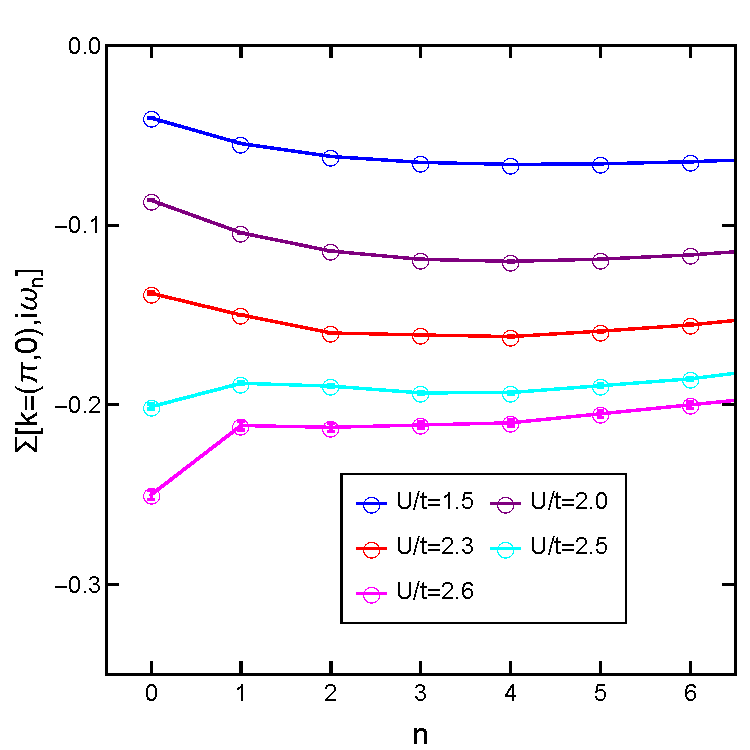
\includegraphics[width=\linewidth]{HF_freq.pdf}
\caption{\label{fig:freqdep}(Color online.) Frequency dependence  of the imaginary part of the self-energy for $T/t=0.1$ at different values of interaction $U/t$ showing a transition from FL ($\rm{Im}\Sigma_k (i\omega_0) >\rm{Im}\Sigma_k (i\omega_1)$) to nFL behavior ($\rm{Im}\Sigma_k (i\omega_0) <\rm{Im}\Sigma_k (i\omega_1)$).}
\end{figure}

\begin{figure}
\centering
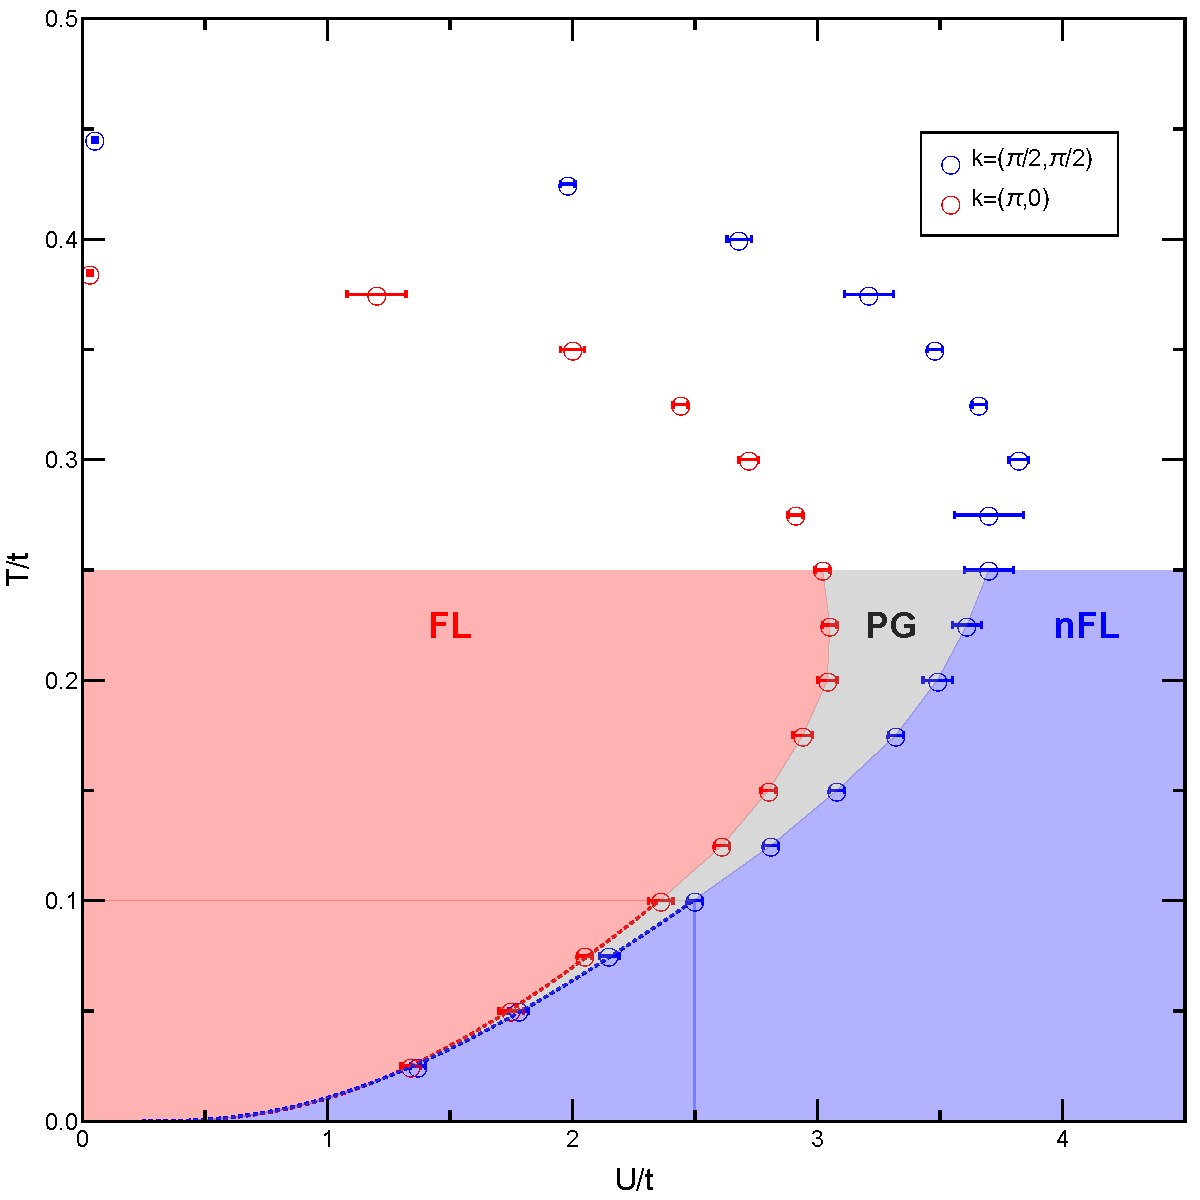
\includegraphics[width=\linewidth]{new_pg_plot.pdf}
\caption{\label{fig:phasediagram}(Color online.) Phase diagram for FL-pseudogap-nFL  crossovers as calculated by $\Sigma$-DDMC. Dotted lines fit data by the functions $T_{an}=a\exp(b/\sqrt{U_{an}})$ and $T_n=a'\exp(b'/\sqrt{U_n})$ with $\{a,b,a',b'\}=\{6.99,-6.51,4.7,-6.08\}$. Full circles represent extrapolated values without error bars.}
\end{figure}


 Central to the success of the $\Sigma$DDMC method is the order by order evaluation of diagrams, the full formalism for which can be found in the recent paper by \v{S}imkovic et al. \onlinecite{simkovic2017determinant}. Summing the full diagrammatic series in terms of the bare propagator $G_0$ and bare interaction, $U$, has the advantage that each order of the series has a separable $U^N$ dependence. The general form for the self-energy series expansion is given by 
\begin{equation}
\Sigma_{\mathrm{k} \sigma}(T,\mu, U) = \sum_{n=1}^{\infty} a_{n, \mathrm{k}\sigma}(T,\mu_{\sigma}-\alpha_{\sigma},\alpha_{\sigma}/U) \, \left(U \xi\right)^{n} , \label{eqn:Sigma_series_gen}
\end{equation}
where $\alpha_{\sigma}$ is a free parameter \cite{rubtsov2005continuous}. At half-filling it is optimal to set $\alpha_{\sigma} =\mu_{\sigma} \equiv U/2$, which leads to all diagrams with self-loop terms as well as all odd order diagrams equaling zero. The resulting series for the self-energy then simplifies to
 \begin{equation}
\Sigma_{\mathrm{k} \sigma}(T, U) = \sum_{n=1}^{\infty} a_{2n, \mathrm{k}\sigma}(T) \, \left(U \xi\right)^{2n}, \label{eqn:Sigma_series}
\end{equation}
 where the coefficients $a_{2n, \mathrm{k}\sigma}$ must be determined for each given temperature. The self-energy can then be analytically evaluated for all $U/t$ values, which trivializes the process of finding the crossovers $U_{an}(T)$ and $U_n(T)$. This reduces the phase space from two-dimensions in $T-U$ to one dimensional, providing results that can readily be evaluated at arbitrary values of $U/t$. 
 
 Using $\Sigma$DDMC we are able to calculate results for the self-energy up to order 12 for high enough temperatures ($T\geq 0.1$) and up to order 10 for temperatures below (($0.025 \leq T\leq 0.1$)). 
 As discussed in Ref.~\cite{simkovic2017determinant} the perturbation expansion risks sampling singular points.  The positions of singularities in the complex plane of the expansion parameter can be identified by means of Dlog Pad\'{e} approximants \cite{baker1961application}. We find at half-filling that there is a singularity on the positive real axis as well as a pair purely imaginary singularities that are equidistant from the origin.
 
 It is believed that the real singularity is related to the metal-insulator-transition. Rigorously identifying what role singularities play in the critical properties of the system remains an open question beyond the present work; one likely answered through knowledge of two particle quantities.\cite{gunnarsson:2015,wu:2017,gunnarsson:2018}
 
 The imaginary singularities come from the fact that we are analyzing a series where every other term is zero. These extra singularities can be eliminated by instead analyzing the equivalent series in terms of the square of the interaction:
 \begin{align}
     \sum_{m=1}^{\infty} a_{m, \mathrm{k}\sigma}(T) \, \left(U^2 \xi^2 \right)^{m}  
 \end{align}
 and taking the square root at the end. The self-energy at a particular temperature $T$ can then be obtained from the Dlog Pad\'{e} approximants for any interaction $U$ within the convergence radius defined by the positive real singularity. It was found that the  crossover interactions $U_n$ and $U_{an}$ are also always within this convergence radius.

 Contrary to DDMC which calculates the extensive partition function, $\Sigma$DDMC samples the self-energy directly in momentum and Matsubara frequency space and is therefore in the thermodynamic limit. Also, $\Sigma$DDMC can restrict itself to simply evaluating the lowest two frequencies at the specific $k$-points required to generate $\Delta\Sigma_{k}$. This is distinct from DMFT methods like DCA which must evaluate all momenta as well as a large range in frequency in order to perform self consistency loops.\cite{georges:1996} This gives the $\Sigma$DDMC yet another computational advantage for tackling this specific problem.
 Additionally, $\Sigma$DDMC provides the freedom to work both in the thermodynamic limit and also on a finite lattice of arbitrary size which permits us to study in detail the role of finite size effects.
  
As temperature is decreased the variance of the Monte Carlo algorithm and thus necessary computational effort increases due to an increasing average real-space spread of vertex configurations.  An added difficulty in going to even lower temperatures is the tabulation and memory storage of the bare Green's function. In this work we do not extend below $\beta t=40$.

To assist in the analysis of data from $\Sigma$DDMC we also perform DCA calculations.  The dynamical cluster approximation is a non-perturbative momentum space variant of cluster DMFT with which we utilize an auxiliary field cluster impurity solver.\cite{ hettler:2000,jarrell:2001,Maier05} 
 It is known that at weak coupling the Hubbard model exhibits strong finite size effects below $T/t=0.2$.\cite{benchmark:2015}  Therefore we only make comparisons to DCA at higher temperatures where currently accessible system sizes are known to provide numerically correct behaviour. \cite{benchmark:2015}

%%%%%%%%%%%%%%
\section{Results}

 Shown in Fig.~\ref{fig:freqdep} are results from $\Sigma$DDMC for the imaginary part of the self energy at the antinodal point on the Fermi surface, for variation in $U/t$. We see that at $U/t=2$, there is an upwards curvature towards $n=0$ suggesting FL behavior. Increasing $U/t$ shows a trend towards nFL behavior.
We observe that $k=(\pi,0)$ is the first momentum to show nFL behaviour but also note that data in Fig.~\ref{fig:freqdep} are obtained from a single numerical result for $a_{2n,k\sigma}(T)$ evaluated for increasing $U/t$ as in Eqn.~(\ref{eqn:Sigma_series}).  It is then straightforward to sweep a range of temperatures to map the phase diagram at half-filling.

 Such a result is shown in Fig.~\ref{fig:phasediagram}, which displays the full $U-T$ phase diagram and is the primary result of this work.  Here we mark the Fermi liquid (FL) region (red shading) where $\Delta \Sigma_{k} >0$ for all momenta, the non-Fermi liquid (nFL) region (blue shading) where $\Delta \Sigma_{k} <0$ for all momenta and the low temperature crossover pseudogap region, PG (grey), between the two.

 One notes at low temperature that both $T_{an}$ and $T_n$ scale exponentially as $T_{an}=a\exp(b/\sqrt{U_{an}})$ and $T_N=a'\exp(b'/\sqrt{U_n})$.  We find fit values $a=6.99$, $b=-6.51$, $a'=4.7$, $b'=-6.08$.  At higher temperatures this exponential scaling ends due to a second sign change in $\Delta \Sigma$. This results in maximal values of $U_{an}/t=3$ at $T/t=0.2$ and a value of $U_n$/t just below $4$ at $T/t=0.25$.

 Understanding the multivalued nature of the crossover is straightforward.  The metric is dependent upon the relative strengths of the lowest two Matsubara frequencies.  In general $\rm{Im}\Sigma_{k}(i\omega_n)$ is a negative valued decaying function, such that at high frequency it should always be the case that ${\rm Im}\Sigma_{k}(i\omega_n)-{\rm Im}\Sigma_{k}(i\omega_{n+1})<0$ and it is only at low frequency that $\Delta \Sigma_{k}$ can be greater than 0.  Since the Matsubara spacing is dependent on temperature, at high enough temperatures the first two frequencies are too large to see the FL state and the metric identifies the crossover to the thermal liquid and not the PG state.  Any correct numerical technique must reproduce Fig.~\ref{fig:phasediagram} in the thermodynamic limit and show both a low-$T$ crossover to the PG state as well as a high-temperature thermal state above $T/t=0.225$.

The results in Fig.~\ref{fig:phasediagram} pose a significant computational challenge for most numerical methods.  To illustrate this, we reduce the $\Sigma$DDMC data from the TDL to a restricted finite sized space. Doing so provides an understanding for the extent of finite size effects.  Fig.~\ref{fig:weakcoupling} (top frame) shows the crossovers  in the $U/t \to 0$ limit as a function of $1/L$ where $L$ is the linear dimension of the system size - here ranging from $L\times L=6\times6 \to 40\times40$.  We see strong finite size effects which in practice might pollute the observed scaling in Fig.~\ref{fig:phasediagram}.  Previous work has shown nearly linear trends\cite{schafer:2015} and this was explained recently as being due to finite size effects which agrees with our observations.\cite{vanloon:2018}  



\begin{figure}
\centering
\includegraphics[width=0.8\linewidth]{fig3a_sept2018.eps}\\
\includegraphics[width=0.8\linewidth]{fig3b_sept2018.eps}
\caption{\label{fig:weakcoupling}(Color online.) \emph{Top}: Crossover temperatures in the weak-coupling limit $U/t\rightarrow 0$ as a function of inverse linear system size $1/L$. Squares represent results in the thermodynamic limit. \emph{Bottom}:
Crossover interaction strengths $U_{an}$ and $U_n$ as a function of inverse linear system size $1/L$ for temperature $T/t=0.1$ (solid lines) and $T/t=0.2$ (dashed lines).}
\end{figure}

\begin{figure}
\centering
\includegraphics[width=\linewidth]{dca-vsw.eps}
\caption{\label{fig:dcavsw}  Imaginary self energy from DCA at nodal(left) and anti-nodal(right) for parameters exhibiting a pseudogap, $U/t=3$, $T/t=0.12$, for increasing cluster sizes $N_c=16,64,72,128,144$. }
\end{figure}

\begin{figure}
\centering
\includegraphics[width=\linewidth]{fig5_redone.eps}
\caption{\label{fig:U3vsT_AN} Results from DCA as a function of temperature for the anti-nodal(Top) and nodal(bottom) crossovers for $N_c=8,32,64,128$. Also shown are several values in the TL obtained by extrapolation in $1/N_c \to 0$.  }
\end{figure}


 In Fig.~\ref{fig:weakcoupling} (bottom frame) we show the finite size effects in the values of $U_n$ and $U_{an}$.  At $T/t=0.1$ finite size effects change the results by $20\to30 \%$, while above $T/t=0.2$ this issue has nearly vanished.  Indeed, previous work \cite{schafer:2015} is in agreement at higher temperatures. 
  We find as well that the onset of strong finite size effects below $T/t=0.2$ restricts many methods from converging results, which we exemplify with the DCA method.
   Guided by $\Sigma$DDMC we work to verify at higher temperature the existence of both the lower and upper crossovers as well as the pseudogapped region which has been reported mostly at higher interaction strength. We present DCA results focused at high temperature where accessible system sizes can provide controlled extrapolations.

 Fig.~\ref{fig:dcavsw} displays DCA results at $U/t=3$ shown at $T/t=0.12$.  The left hand frame is for the nodal point which shows FL behaviour at all system sizes.  The antinodal point instead shows a behavioural change as a function of $N_c$ as the system size increases.  This is suggestive of a nFL behavior at $k=(\pi,0)$ for large systems in agreement with Fig.~\ref{fig:phasediagram} from $\Sigma$DDMC.  However, we notice substantial differences in the antinodal region between $N_c=64$ and $128$ at this temperature.  The situation worsens as temperature decreases as correlation lengths increase. 

 This leads us to explore fixed $U/t$ cuts in temperature.  Results are shown in Fig.~\ref{fig:U3vsT_AN}.  Guided by previous cDMFT and D$\Gamma$A studies\cite{Schaefer:2016,park:2008} and by these new $\Sigma$DDMC results we focus on the predicted turning points of Fig.~\ref{fig:phasediagram} which occur near $U/t=3$ at $T/t=0.2$ for the antinodal wavevector and at $U/t=4$ at $T/t=0.25$ for the nodal wavevector.

 Fig.~\ref{fig:U3vsT_AN} demonstrates $\Delta \Sigma_{k}$ as a function of $T/t$ for $N_c=8,32,64,128$ in the antinodal (top frame) and nodal (bottom frame) regions. Both momenta for small clusters see FL behaviour at low temperature and a single crossover at high temperatures.  As system size is increased above $N_c=64$ we see a substantial dependence on system size at low $T/t$ and weaker finite size effects at high temperature.  We also see two sign changes for $N_c=64$ and $128$ with a region in between becoming progressively more narrow with increased system size.  In both frames, we have a target provided by $\Sigma$DDMC, the vertical black dashed line at $U/t=3$, $T/t=0.2$ and in the lower frame at $U/t=4$ at $T/t=0.25$.  To obtain results in the thermodynamic limit we perform linear extrapolation in the system size as $1/N_c \to 0$ for the $\Delta \Sigma_{k}$ from our DCA calculations.  In both cases, as predicted by $\Sigma$DDMC, these points in the phase diagram are at the cusp of a FL/nFL crossover suggested by convergence of the extrapolation of $\Delta \Sigma_{k} \to 0$. It is clear that these points are in a region where the low temperature PG and high temperature thermal crossovers merge. 

%%%%%%%%%%%%%%

\section{Conclusions}
In summary, we provide a rigorous and controlled representation of the metal-pseudogap-insulator crossover.  We find at low temperatures exponential trends for both the pseudogap and insulator onsets, defined by $T_{an}=a\exp(b/\sqrt{U_{an}})$ and $T_n=a'\exp(b'/\sqrt{U_n})$ with $\{a,b,a',b'\}=\{6.99,-6.51,4.7,-6.08\}$. 

\section{Acknowledgments}
This work was supported by the Simons Collaboration on the Many-Electron Problem, the National Science Foundation under the grant DMR-1720465, and the MURI Program ``Advanced quantum materials - a new frontier for ultracold atoms" from AFOSR. JPFL was funded by NSERC and computational resources were provided by Compute Canada.

% \begin{figure}
% \centering
% \includegraphics[width=\linewidth]{U3_extrap.eps}\\
% \includegraphics[width=\linewidth]{U4_extrap.eps}
% \caption{\label{fig:dca_supplemental} (SUPPLEMENTAL) DCA extrapolations for supplemental.}
% \end{figure}



\bibliographystyle{apsrev4-1}
\bibliography{refs.bib}

\end{document}
